\chapter{线性映射矩阵表示}

在上一讲的讨论中我们定义了线性映射的基本概念,讨论了由其定义直接引出的性质. 本节我们将深入讨论线性映射像空间与核空间之间的关联,从而引出我们目前为止最核心的概念——同构,因为同构使得我们研究的抽象层次更上一层,最后我们将在这抽象的制高点获得最具象的表达形式——矩阵,介绍线性映射矩阵表示的定义,以及这一定义下线性映射与矩阵的一一对应关系,从而使得我们后续的研究都可以基于具象的矩阵. 除此之外,本节在讨论了同构之后将引入线性空间的直积作为应用,完整地展示从线性空间的定义到性质研究到利用线性映射研究进一步的性质的思路.

\section{线性映射矩阵表示}

作为准备,我们首先需要引入矩阵的概念:
\begin{definition}
    域$\mathbf{F}$中的$m\times n$个元素$a_{ij}\enspace(i=1,\ldots,m,\enspace j=1,\ldots,n)$排成$m$行$n$列的矩形数表,称为域$\mathbf{F}$上的一个$m\times n$矩阵,记作
    \[A=\begin{pmatrix}
            a_{11} & a_{12} & \cdots & a_{1n} \\
            a_{21} & a_{22} & \cdots & a_{2n} \\
            \vdots & \vdots & \ddots & \vdots \\
            a_{m1} & a_{m2} & \cdots & a_{mn}
        \end{pmatrix}\]
    或简记为$(a_{ij})_{m\times n}$,其中$a_{ij}$表示矩阵$A$的第$i$行第$j$列的元素.
\end{definition}

我们有一些常用的矩阵,例如零矩阵,即所有元素均为0的矩阵,通常记为$O$;单位矩阵也十分常见,它表示对角线上元素为1,其余元素为0的矩阵,通常记为$E$(若已知阶数为$n$也可特别记为$E_n$).

除此之外,我们通常记域$\mathbf{F}$上的$m\times n$矩阵全体为$\mathbf{F}^{m\times n}$或$\mathbf{M}_{m\times n}(\mathbf{F})$. 当$m=n$时矩阵称为方阵,域$\mathbf{F}$上全体$n$阶矩阵(或称$n$阶方阵)记为$\mathbf{F}^{n\times n}$或$\mathbf{M}_n(\mathbf{F})$.

在了解矩阵的定义之后,我们可以引入线性映射矩阵表示的概念. 经过前面大量的关于坐标同构的铺垫之后,想必读者对于如何将抽象的映射转化为矩阵有一个大致的思路:事实上,我们可以将矩阵视为多个$\mathbf{R}^n$中的列向量拼在一起得到的方块,那么如何得到这些$\mathbf{R}^n$中的列向量呢?想必是某些向量在线性映射到达空间的一组基下的坐标. 于是我们很自然地可以接受下面的定义:
\begin{definition}\label{def:7:线性映射矩阵表示}
    设$B_1=\{\varepsilon_1,\varepsilon_2,\ldots,\varepsilon_n\}$是$V_1(\mathbf{F})$的基,$B_2=\{\alpha_1,\alpha_2,\ldots,\alpha_m\}$是$V_2(\mathbf{F})$的基. 则线性映射$\sigma \in \mathcal{L}(V_1,V_2)$被它作用于基$B_1$的像
    \[\sigma(B_1)=\{\sigma(\varepsilon_1),\sigma(\varepsilon_2),\ldots,\sigma(\varepsilon_n)\}\]
    所唯一确定,而$\sigma(B_1)$是$V_2$的子空间,于是其中元素都可以被基$B_2$线性表示,即
    \[ \begin{cases} \begin{aligned}
                \sigma(\varepsilon_1) & = a_{11}\alpha_1+a_{21}\alpha_2+\cdots+a_{m1}\alpha_m \\
                \sigma(\varepsilon_2) & = a_{12}\alpha_1+a_{22}\alpha_2+\cdots+a_{m2}\alpha_m \\
                                      & \vdotswithin{=}                                       \\
                \sigma(\varepsilon_n) & = a_{1n}\alpha_1+a_{2n}\alpha_2+\cdots+a_{mn}\alpha_m
            \end{aligned} \end{cases} \]

    我们将$\sigma(B_1)=\{\sigma(\varepsilon_1),\sigma(\varepsilon_2),\ldots,\sigma(\varepsilon_n)\}$关于基$B_2$的坐标排列成矩阵$\mathbf{M}(\sigma)$,即
    \[\mathbf{M}(\sigma)=\begin{pmatrix}
            a_{11} & a_{12} & \cdots & a_{1n} \\
            a_{21} & a_{22} & \cdots & a_{2n} \\
            \vdots & \vdots & \ddots & \vdots \\
            a_{m1} & a_{m2} & \cdots & a_{mn}
        \end{pmatrix}\]
    我们称$\mathbf{M}(\sigma)$为$\sigma$在基$B_1$和$B_2$下的矩阵表示,有时也称线性映射在基下的表示矩阵.
\end{definition}

更通俗来说,线性映射矩阵表示就是将线性映射在一组基上的像在另一组基下的坐标表示按列排列得到的结果. 这一整体过程我们也可以用如下记号表示:
\begin{equation}\label{eq:7:线性映射矩阵表示}
    (\sigma(\varepsilon_1),\sigma(\varepsilon_2),\ldots,\sigma(\varepsilon_n))=(\alpha_1,\alpha_2,\ldots,\alpha_m)\mathbf{M}(\sigma).
\end{equation}

根据定义我们直接有如下简单的观察:
\begin{enumerate}
    \item 线性映射矩阵表示的结果是一个$m\times n$矩阵,其中$m$是到达空间的维数,$n$是出发空间的维数,特别注意此处有个次序的颠倒,务必区分清楚;

    \item 若$\sigma$在基下矩阵表示为$A=(a_{ij})_{m\times n}$,在出发空间的基的第$i$个向量在到达空间基下的坐标为$(a_{1i},a_{2i},\ldots,a_{mi})$,即矩阵$A$的第$i$列,或写为$\sigma(\varepsilon)=a_{1i}\alpha_1+a_{2i}\alpha_2+\cdots+a_{mi}\alpha_m$.
\end{enumerate}

想必有很多读者会心存疑惑:为什么我们要这么定义线性映射的矩阵表示呢?我们将在下一小节说明线性映射构成的线性空间与矩阵构成线性空间的同构时解释这一点. 现在先让我们完成以下几个例题熟悉定义:
\begin{example}\label{ex:7:矩阵表示1}
    已知$\sigma \in \mathcal{L}(\mathbf{R}^3,\mathbf{R}^3)$且$\sigma(x_1,x_2,x_3)=(x_1+x_2,x_1-x_3, x_2)$
    \begin{enumerate}
        \item 求$\sigma$的像空间和核空间;

        \item 求$\sigma$关于$\mathbf{R}^3$自然基的矩阵.
    \end{enumerate}
\end{example}

\begin{solution}
    \begin{enumerate}
        \item 求像空间和核空间的方法我们在之前已经介绍过,我们为了计算方便取$\mathbf{R}^3$的自然基$e_1,e_2,e_3$计算有:
              \[\im\sigma=\spa(\sigma(e_1),\sigma(e_2),\sigma(e_3))=\spa((1,1,0),(1,0,1),(0,-1,0))=\mathbf{R}^3\]
              对于核空间,解方程$\sigma(\alpha)=0$即可. 我们也可以用更简洁的方式书写:
              \[\ker\sigma=\{(x_1,x_2,x_3)\mid \sigma(x_1,x_2,x_3)=(0,0,0)\}=\{(0,0,0)\}\]
              即方程只有零解,核空间可以记为$\ker\sigma=\{0\}$(只含零元的空间的一般记法).

        \item 我们根据\autoref{def:7:线性映射矩阵表示},应先写出$\sigma$在出发空间一组基(按题目要求是$\mathbf{R}^3$自然基)下的像,并将像表示为到达空间基(按题目要求是$\mathbf{R}^3$自然基)的线性组合,即
              \begin{gather*}
                  \sigma(e_1)=(1,1,0)=e_1+e_2=(e_1,e_2,e_3)\begin{pmatrix}
                      1 \\ 1 \\ 0
                  \end{pmatrix} \\
                  \sigma(e_2)=(1,0,1)=e_1+e_3=(e_1,e_2,e_3)\begin{pmatrix}
                      1 \\ 0 \\ 1
                  \end{pmatrix} \\
                  \sigma(e_3)=(0,-1,0)=-e_2=(e_1,e_2,e_3)\begin{pmatrix}
                      0 \\ -1 \\ 0
                  \end{pmatrix}
              \end{gather*}
              接下来我们把坐标依次按列称矩阵就得到了本题需要求解的矩阵:
              \[\mathbf{M}(\sigma)=\begin{pmatrix}
                      1 & 1 & 0  \\
                      1 & 0 & -1 \\
                      0 & 1 & 0
                  \end{pmatrix}\]
    \end{enumerate}
\end{solution}

有趣的是,在结合我个人的学习经历以及过往辅学的经验后,我总结出了第二问的一种常见的错误解法,这里我需要加粗强调,下面这种解法是\textbf{完全错误的!!!}这里展示这一解法是为了让读者将前面所学的知识完全厘清:

\begin{solution}
    (\textbf{\songti 错误解法!!!})$\sigma(x_1,x_2,x_3)=(x_1+x_2,x_1-x_3, x_2)=(x_1,x_2,x_3)\begin{pmatrix}
            1 & 1  & 0 \\
            1 & 0  & 1 \\
            0 & -1 & 0
        \end{pmatrix}$
\end{solution}

我们惊奇地发现,这一结果和我们前面得到的标准答案在向量的排列方式上发生了变化,即标准答案的1、2、3行变为了这里的1、2、3列,我们需要强调两点:
\begin{enumerate}
    \item 为什么这种解法是错误的:我们可以直接比较\autoref{eq:7:线性映射矩阵表示} 和这一解法中,\autoref*{eq:7:线性映射矩阵表示} 的等号左边是$n$个向量在$\sigma$下的像,而上述解法$\sigma(x_1,x_2,x_3)$只是$\sigma$在一个向量下的像,这显然是不一样的!!!同样,等号右边括号内\autoref*{eq:7:线性映射矩阵表示} 是到达空间的一组基,而上述解法中仍然只是一个向量. 我们从未定义过这样解题的结果是什么,所以千万不能做这种无意义的事!!!

          容易导致混淆的原因可能在于$(x,y,z)$向量是排列成一行的,可能看起来和$(e_1,e_2,e_3)$有点相似,但如果我们将后者拆分成$((1,0,0),(0,1,0),(0,0,1))$,你还会混淆吗?

    \item 为什么会出现行列互换这样的错误:事实上
          \[\sigma(x,y,z)=\sigma(xe_1+ye_2+ze_3)=x\sigma(e_1)+y\sigma(e_2)+z\sigma(e_3)=(x,y,z)\begin{pmatrix}
                  \sigma(e_1) \\ \sigma(e_2) \\ \sigma(e_3)
              \end{pmatrix},\]
          这里将$\sigma(e_1),\sigma(e_2),\sigma(e_3)$的结果按行排列成矩阵,而标准答案是将$\sigma(e_1),\sigma(e_2),\sigma(e_3)$在$\mathbf{R}^3$自然基下的坐标按列排列成矩阵,回忆$\mathbf{R}^n$向量在自然基下坐标是其本身这一性质,标准答案就是将$\sigma(e_1),\sigma(e_2),\sigma(e_3)$按列排列成矩阵,由此我们解释了行列互换发生的原因.
\end{enumerate}

这也就是为什么我强调读者不要参考教材102页例3求解像空间的方法来求解像空间——很容易导致这里矩阵表示犯这样的错误,并且容易导致初学时无法区分求解像空间和线性映射矩阵表示的方法. 在这里我必须再次强调:在没有完全熟练掌握这些概念和方法前,不要乱用方法!!!

还需要强调的一点是,教材121页例2中介绍了旋转变换的矩阵表示,即$\mathbf{R}^2$中向量绕原点按逆时针方向旋转$\theta$角的变换关于$\mathbf{R}^2$的自然基的矩阵表示为
\[\mathbf{M}(\sigma)=\begin{pmatrix}
        \cos\theta & -\sin\theta \\
        \sin\theta & \cos\theta
    \end{pmatrix}\]
这一形式可以记忆,在之后会多次出现.

\section{$\mathcal{L}(V_1,V_2)$与矩阵线性空间的同构}

本节我们将通过说明$\mathcal{L}(V_1,V_2)$与矩阵构成的线性空间的同构来解释为什么我们要这么定义线性映射的矩阵表示. 为了达到这一目标,我们首先需要证明这一同构.

\subsection{矩阵的加法和数乘}

回忆我们定义

本节我们将完善上一讲中同构的例子的细节,即若$\dim V_1(\mathbf{F})=m$,$\dim V_2(\mathbf{F})=n$,则$\mathcal{L}(V_1,V_2) \cong \mathbf{F}^{m \times n}$,其中$\mathbf{F}^{m \times n}$表示全体$m\times n$矩阵构成的线性空间.

要证明这一结论,首先要说明全体$m\times n$矩阵关于某种运算的确构成线性空间,这里的运算——即矩阵的加法和数乘还需要我们来定义. 我们有一个非常自然的想法——既然$V_1\to V_2$的全体线性映射关于线性映射加法和数乘构成线性空间,那么我们也许可以利用线性映射加法与数乘运算的矩阵表示来定义加法和数乘运算.

我们首先回顾线性映射的加法和数乘运算:设$\sigma,\tau\in \mathcal{L}(V_1,V_2)$,规定$\sigma$与$\tau$之和及$\lambda$与$\sigma$的数乘$\lambda\sigma$分别为
\begin{gather*}
    (\sigma+\tau)(\alpha)=\sigma(\alpha)+\tau(\alpha),\enspace\forall\alpha\in V_1 \\
    (\lambda\sigma)(\alpha)=\lambda(\sigma(\alpha)),\enspace\forall\alpha\in V_1
\end{gather*}

回顾线性映射的矩阵表示,我们实际上是要计算出线性映射在出发空间一组基下的像在到达空间一组基下的坐标然后按列排列. 我们取$V_1$的基$B_1=\{\varepsilon_1,\varepsilon_2,\ldots,\varepsilon_n\}$,$V_2$的基$B_2=\{\alpha_1,\alpha_2,\ldots,\alpha_m\}$,假设$\sigma$和$\tau$在$B_1$和$B_2$下的矩阵分别为$A=(a_{ij})_{m\times n}$和$B=(b_{ij})_{m\times n}$,则
\begin{gather*}
    \sigma(\varepsilon_i)=a_{1i}\alpha_1+a_{2i}\alpha_2+\cdots+a_{mi}\alpha_m \\
    \tau(\varepsilon_i)=b_{1i}\alpha_1+b_{2i}\alpha_2+\cdots+b_{mi}\alpha_m.
\end{gather*}
因此
\[(\sigma+\tau)(\varepsilon_i)=(a_{1i}+b_{1i})\alpha_1+(a_{2i}+b_{2i})\alpha_2+\cdots+(a_{mi}+b_{mi})\alpha_m,\enspace i=1,2,\ldots,n\]
即$(\sigma+\tau)$矩阵表示$\mathbf{M}(\sigma+\tau)$的第$i$列元素为$A$和$B$的第$i$列对应元素相加. 由于$i$是任取的,因此$(\sigma+\tau)$的矩阵表示每一列都是$A$和$B$同一列对应元素相加,实际上对于整个矩阵而言就是矩阵相同位置元素相加,即
\begin{align*}
    \mathbf{M}(\sigma+\tau) & =\begin{pmatrix}
                                   a_{11}+b_{11} & a_{12}+b_{12} & \cdots & a_{1n}+b_{1n} \\
                                   a_{21}+b_{21} & a_{22}+b_{22} & \cdots & a_{2n}+b_{2n} \\
                                   \vdots        & \vdots        & \ddots & \vdots        \\
                                   a_{m1}+b_{m1} & a_{m2}+b_{m2} & \cdots & a_{mn}+b_{mn}
                               \end{pmatrix}     \\
                            & \triangleq\begin{pmatrix}
                                            a_{11} & a_{12} & \cdots & a_{1n} \\
                                            a_{21} & a_{22} & \cdots & a_{2n} \\
                                            \vdots & \vdots & \ddots & \vdots \\
                                            a_{m1} & a_{m2} & \cdots & a_{mn}
                                        \end{pmatrix} + \begin{pmatrix}
                                                            b_{11} & b_{12} & \cdots & b_{1n} \\
                                                            b_{21} & b_{22} & \cdots & b_{2n} \\
                                                            \vdots & \vdots & \ddots & \vdots \\
                                                            b_{m1} & b_{m2} & \cdots & b_{mn}
                                                        \end{pmatrix} \\
                            & =\mathbf{M}(\sigma)+\mathbf{M}(\tau).
\end{align*}
式中$\triangleq$表示定义,即定义矩阵加法为矩阵对应元素相加. 同理,我们也可以通过线性映射的数乘定义矩阵数乘运算如下:
\[\mathbf{M}(\lambda\sigma)=\begin{pmatrix}
        \lambda a_{11} & \lambda a_{12} & \cdots & \lambda a_{1n} \\
        \lambda a_{21} & \lambda a_{22} & \cdots & \lambda a_{2n} \\
        \vdots         & \vdots         & \ddots & \vdots         \\
        \lambda a_{m1} & \lambda a_{m2} & \cdots & \lambda a_{mn}
    \end{pmatrix}\triangleq\lambda\begin{pmatrix}
        a_{11} & a_{12} & \cdots & a_{1n} \\
        a_{21} & a_{22} & \cdots & a_{2n} \\
        \vdots & \vdots & \ddots & \vdots \\
        a_{m1} & a_{m2} & \cdots & a_{mn}
    \end{pmatrix}=\lambda\mathbf{M}(\sigma).\]
事实上这非常符合我们对于矩阵加法和数乘的幻想,即矩阵加法就是对应元素相加,矩阵数乘就是对应元素乘以一个数.

在利用线性映射的加法和数乘定义了非常自然的矩阵加法和数乘后,我们需要验证$m\times n$矩阵全体关于这两种运算构成线性空间. 这里我们只需回顾线性空间运算的八条要求然后逐一验证即可,实际上非常简单,因此不在此赘述.

\subsection{同构的说明}

在上一小节中我们定义了矩阵的加法和数乘运算,也验证了全体$m\times n$矩阵关于这两种运算构成线性空间$\mathbf{F}^{m\times n}$,接下来我们需要讨论的是对于$n$维线性空间$V_1$和$m$维线性空间$V_2$,$\mathcal{L}(V_1,V_2)$与$\mathbf{F}^{m\times n}$的同构. 即我们需要定义一个线性双射$\varphi:\mathcal{L}(V_1,V_2)\to\mathbf{F}^{m\times n}$. 事实上我们只需要很自然地利用线性映射矩阵表示定义,即定义
\[\varphi(\sigma)=\mathbf{M}(\sigma),\]
也就是说$\varphi$将线性映射$\sigma$映射为其矩阵表示. 接下来需要验证$\varphi$是线性双射.
\begin{enumerate}
    \item 线性性是显然的,因为根据矩阵加法和数乘的定义,我们有
          \begin{gather*}
              \varphi(\sigma+\tau)=\mathbf{M}(\sigma+\tau)=\mathbf{M}(\sigma)+\mathbf{M}(\tau)=\varphi(\sigma)+\varphi(\tau) \\
              \varphi(\lambda\sigma)=\mathbf{M}(\lambda\sigma)=\lambda\mathbf{M}(\sigma)=\lambda\varphi(\sigma).
          \end{gather*}

    \item 双射也是显然的:
          \begin{enumerate}
              \item 对于单射性,我们考察$\varphi$的核空间$\ker\varphi$中的元素$\sigma$,即$\sigma$在基下的矩阵表示为零矩阵,那么$\sigma$必然为零映射,因为它将所有基映射为0,故必然将所有出发空间元素映射为0,因此核空间为$\{0\}$,单射成立;

              \item 对于满射性,我们需要为任意$m\times n$矩阵$(a_{ij})_{m\times n}$找到一个线性映射,使得这一矩阵为这一线性映射在基下的矩阵表示. 事实上,给定基和矩阵表示,我们就知道了线性映射在出发空间的基下的像——因为给定到达空间的基和矩阵就给定了线性映射在出发空间的基在到达空间的基下的坐标. 然后根据\autoref{thm:5:线性映射构造} 知我们一定能找到这一映射,故满射性成立.
          \end{enumerate}
\end{enumerate}

由此我们证明了$\mathcal{L}(V_1,V_2)\cong\mathbf{F}^{m\times n}$. 而我们很容易知道,$\mathbf{F}^{m\times n}$的维数为$mn$. 事实上对于矩阵关于矩阵加法和数乘构成的线性空间,我们有如下一组常用基:$E_{ij}(i=1,\cdots,m,j=1,\cdots,n)$,其中每个$E_{ij}$为第$i$行$j$列元素为1,其余元素全为0的矩阵. 例如对于$\mathbf{F}^{2\times 3}$,根据前面的描述我们可以写出其常用基为:
\[E_{11}=\begin{pmatrix}
        1 & 0 & 0 \\
        0 & 0 & 0
    \end{pmatrix},\enspace E_{12}=\begin{pmatrix}
        0 & 1 & 0 \\
        0 & 0 & 0
    \end{pmatrix},\enspace E_{13}=\begin{pmatrix}
        0 & 0 & 1 \\
        0 & 0 & 0
    \end{pmatrix},\]
\[E_{21}=\begin{pmatrix}
        0 & 0 & 0 \\
        1 & 0 & 0
    \end{pmatrix},\enspace E_{22}=\begin{pmatrix}
        0 & 0 & 0 \\
        0 & 1 & 0
    \end{pmatrix},\enspace E_{23}=\begin{pmatrix}
        0 & 0 & 0 \\
        0 & 0 & 1
    \end{pmatrix},\]
事实上,我们很容易验证这样的常用基的确是线性空间$\mathbf{F}^{m\times n}$的一组基,因为它们显然是线性无关的,且张成整个空间(请读者自行验证),然后我们也知道这样的常用基中矩阵有$m\times n$个,由此我们也得到了$\dim\mathcal{L}(V_1,V_2)=mn$. 当然我们还可以有另一种理解方式,如果读者已经学习过编程中二维数组的概念,事实上二维数组在计算机中的存储形式是一行存完接着马上存下一行,因此事实上我们可以将二维数组看作是一个长为$m\times n$的一维数组(方法就是第一行写完后在同一行马上接着写第二行元素,写完后在同一行接着写第三行元素,依此类推),因此我们也可以理解为$\mathbf{F}^{m\times n}$和$\mathbf{F}^{mn}$是没有区别的(容易验证是同构的),因此$\dim\mathbf{F}^{m\times n}=mn$.

\section{线性映射的不变子空间}

回顾我们接下来讨论的目标,即找到一组基使得线性变换在这组基下的表示更简单. 设$\sigma\in\mathcal{L}(V)$,如果$V$有直和分解
\begin{equation}\label{eq:18:直和分解}
    V=U_1\oplus U_2\oplus\cdots\oplus U_m,
\end{equation}
其中每个$U_i$都是$V$的真子空间,那么我们对于$\sigma$的研究可以分别在各个$U_i$上进行. 这其中的基本原理在于直觉告诉我们(并且实际上通常而言)更低维的空间处理起来应当更为简单,事实上我们后面的很多工作都是在找这样的分解.

为了在低维空间上进行研究,我们需要引入一个新的概念,即$\sigma$在$U_i$下的限制映射$\sigma\vert_{U_i}$. 我们给出标准的定义如下:
\begin{definition} \index{xianxingyingshe!xianzhi@限制 (restriction map)}
    设$V$是数域$\mathbf{F}$上的线性空间,$\sigma\in\mathcal{L}(V)$,我们在$V$的子空间$U$上定义映射$\sigma\vert_U$如下:
    \[\sigma\vert_U:U\to V,\enspace\sigma\vert_U(\alpha)=\sigma(\alpha),\enspace\forall \alpha\in U,\]
    则称$\sigma\vert_U$是$\sigma$在$U$上的\term{限制映射}.
\end{definition}

``限制''一词十分形象(如下图所示),因为限制映射就是将原映射的定义域限制在更小的范围内,但原定义域上的映射值保持不变.
\begin{figure}[H]
    \centering
    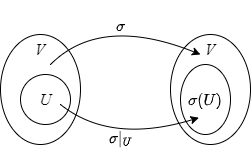
\includegraphics[scale=0.7]{figs/18-1.png}
\end{figure}

但是我们需要注意,\autoref{eq:18:直和分解} 这一分解应当满足一个基本的条件,就是$\sigma$应当把每个$U_i$仍然映射到$U_i$本身,否则我们在讨论$\sigma\vert_{U_i}$的时候它不是一个线性变换,这与我们讨论的主题不一致,即我们希望限制映射$\sigma\vert_{U_i}$是一个线性变换(是$\mathcal{L}(U_i)$中的元素),我们称之为\term{限制线性变换}\index{xianxingbianhuan!xianzhi@限制线性变换 (restriction operator)}.

事实上,满足$\sigma\vert_{U_i}\in\mathcal{L}(U_i)$的子空间$U_i$非常重要,我们需要给予它一个定义:
\begin{definition}
    设$\sigma\in \mathcal{L}(V)$,若$V$的子空间$U$满足$\forall \alpha\in U,\enspace \sigma(\alpha)\in U$,则称$U$是$\sigma$的\term{不变子空间}\index{xianxingkongjian!zi!bubian@不变子空间 (invariant subspace)},或称$U$在$\sigma$下不变,简称为$\sigma$-子空间.
\end{definition}
即不变子空间中的每一个向量经过映射后仍在这一空间中,因此这里的``不变''的含义也是非常直观的. 根据定义我们可以验证或者求解一些很简单的不变子空间. 教材例5.3给出了四个常见的不变子空间的例子,分别是两个平凡子空间和映射的像与核,验证非常简单,此处不赘述. 教材8.20还给出了$p$为多项式时,$\ker p(\sigma)$和$\im p(\sigma)$也为$\sigma$的不变子空间. 我们这里也简要书写一下,供读者熟悉如何利用定义验证不变子空间:
\begin{example}
    若$\sigma\in\mathcal{L}(V)$且$p\in\mathbf{F}[x]$为多项式,则$\ker p(\sigma)$和$\im p(\sigma)$在$\sigma$下不变.
\end{example}

\begin{proof}
    我们只需验证$\ker p(\sigma)$和$\im p(\sigma)$中的元素经过$\sigma$映射后仍在这一空间中即可.
    \begin{enumerate}
        \item $\forall \alpha\in \ker p(\sigma),\enspace p(\sigma)\alpha=0$,因此
              \[(p(\sigma))(\sigma(\alpha))=\sigma(p(\sigma)\alpha)=\sigma(0)=0,\]
              即$\sigma(\alpha)\in \ker p(\sigma)$,因此$\ker p(\sigma)$在$\sigma$下不变;

        \item $\forall \alpha\in \im p(\sigma),\enspace \exists \beta\in V,\enspace \alpha=p(\sigma)\beta$,因此
              \[\sigma(\alpha)=\sigma(p(\sigma)\beta)=p(\sigma)(\sigma(\beta))\in \im p(\sigma),\]
              即$\im p(\sigma)$在$\sigma$下不变.
    \end{enumerate}
    事实上,对于$\ker p(\sigma)$,我们有
    \[ p(\sigma)(\alpha)=p(\sigma)\alpha=p(\sigma(\alpha))=p(0)=0,\]
    因此$\sigma(\alpha)\in \ker p(\sigma)$,即$\ker p(\sigma)$在$\sigma$下不变. 对于$\im p(\sigma)$,我们有
    \[\forall \alpha\in \im p(\sigma),\enspace \exists \beta\in V,\enspace \alpha=p(\sigma)\beta,\]
    因此
    \[\sigma(\alpha)=\sigma(p(\sigma)\beta)=p(\sigma)\sigma(\beta)\in \im p(\sigma),\]
    即$\im p(\sigma)$在$\sigma$下不变.
\end{proof}


\vspace{2ex}
\centerline{\heiti \Large 内容总结}

本节我们重点讨论了线性映射像空间和核空间之间的关联,核心定理就是线性映射基本定理,一方面其证明使用的``设小扩大''的思想十分常见,另一方面它的结论也是相当重要的,它将线性映射的核空间和像空间的维数联系起来,是将来讨论线性方程组一般理论的重要工具,也可以由此导出出发空间、到达空间维数相同时,单射、满射、双射的关联. 除此之外,我们也基于像空间、核空间本身的性质讨论了它们更为复杂的关联,在这些结论的证明中我们能掌握很多基本技巧,如基于像空间、核空间定义的直和的证明、包含关系的证明等,并且综合利用了线性空间维数公式以及本讲介绍的线性映射基本定理,因此很适合作为加深对概念、方法理解运用的例子.

最后我们讨论了线性空间同构的概念,同构映射保持线性相关性的特点,以及通过维数判定有限维线性空间同构的简便方法. 同构是线性空间之间的等价关系,它将线性空间按维数划分为不同的等价类,从而将任意$n$维线性空间的研究转化为对向量空间$\mathbf{R}^n$的研究——事实上本节最后一个例子中构造同构映射的方法就已经体现了这一点的优越性. 同时这也表明线性空间结构的最关键因素就是维数,线性空间之间最本质的差别就是维数不同——这便回应了上一讲开头引言部分的问题. 一组基中的元素是向量还是多项式还是函数并不重要,重要的是只要它们维数相同,我们就可以遮蔽掉元素的差别——因为它们都可以通过坐标映射同构于$\mathbf{R}^n$,因此一切线性空间在坐标作用下都变成了向量空间,变成了最直观的可以用一个一个数字写出来的向量,我们便可以基于此将所有无论多么抽象的线性映射也表示成能用一个一个数字写出来的东西——这就是矩阵. 在有了线性映射的矩阵表示后,我们便可以将抽象的研究都转化为具象的矩阵运算,这一思想我们将在介绍完需要的工具——矩阵运算以及行列式之后深入讨论,届时我们将分别以抽象的线性映射理论和矩阵理论叙述大量的结论,探寻利用二者研究线性代数问题的过程的关联与差异.

\vspace{2ex}
\centerline{\heiti \Large 习题}

\vspace{2ex}
It is not so much whether a theorem is useful that matters, but how elegant it is.
\begin{flushright}
    ——S.Ulam
\end{flushright}

\centerline{\heiti A组}
\begin{enumerate}
    \item 证明:同构映射的逆、复合仍然是同构映射.
\end{enumerate}

\centerline{\heiti B组}
\begin{enumerate}
    \item 设$\sigma(p(x))=p'(x)$(求导),$\forall p(x) \in \mathbf{R}[x]_n$.
          \begin{enumerate}
              \item 证明:$\sigma$是$\mathbf{R}[x]_n$上的线性变换;

              \item 求$\sigma$的值域和$r(\sigma)$,说明$\sigma$是否可逆;

              \item 求$\sigma$的核及其维数;

              \item 求$r(\sigma)+\dim\ker\sigma$,问:$\mathbf{R}[x]_n=\ker\sigma+\im \sigma$是否成立.
          \end{enumerate}

    \item 设$V$为有限维线性空间,$T\in \mathcal{L}(V,V)$且$T$不是恒等变换也不是零变换,问:下列情况是否可能发生?如果可能请举例,不可能请说明理由.
          \begin{enumerate}
              \item $\im T \cap \ker T = \{0\}$;

              \item $\im T \subseteq \ker T$;

              \item $\ker T = \im T$;

              \item $\ker T \subseteq \im T$.
          \end{enumerate}

    \item 若$\sigma_1,\sigma_2\in \mathcal{L}(V,V)$,判断下列说法是否正确,正确请给出证明,反之给出反例:
          \begin{enumerate}
              \item 由$r(\sigma)+\dim\ker\sigma=n$可知$V=\ker\sigma+\im \sigma$;

              \item 若有$\im T \cap \ker T = \{0\}$,则$V=\ker\sigma+\im \sigma$成立;

              \item 因为$\forall \alpha \in V$有$(\sigma_1+\sigma_2)(\alpha)=\sigma_1(\alpha)+\sigma_2(\alpha)$,所以$(\sigma_1+\sigma_2)(V)=\sigma_1(V)+\sigma_2(V)$;

              \item $(I-\sigma)(V)+\sigma(V)=V$,其中$I$为恒等映射.
          \end{enumerate}

    \item 已知$V$为有限维线性空间,$\sigma\in \mathcal{L}(V,V)$,且$\ker\sigma=\im \sigma$,证明:
          \begin{enumerate}
              \item $n$为偶数;

              \item 存在$V$的一组基$\alpha_1,\ldots,\alpha_n$使得
                    \[\sigma(\alpha_1,\ldots,\alpha_n)=(\alpha_1,\ldots,\alpha_n)\begin{pmatrix}
                            0 & E_{\frac{n}{2}} \\ 0 & 0
                        \end{pmatrix}.\]
          \end{enumerate}

    \item 设$V(\mathbf{R})$是线性空间,$\sigma$是$V(\mathbf{R})$到$\mathbf{R}^3$的同构映射,且$\sigma(\alpha_1)=(1,0,1),\enspace\allowbreak\sigma(\alpha_2)=(-2,1,0),\enspace\allowbreak\sigma(\alpha_3)=(-3,2,1),\enspace\allowbreak\sigma(\alpha_4)=(1,1,2)$.
          \begin{enumerate}
              \item $\alpha_1$在$\spa(\alpha_2,\alpha_3)$中吗?

              \item 设$W_1=\spa(\alpha_1,\alpha_2),\enspace W_2=\spa(\alpha_3,\alpha_4)$,求$W_1\cap W_2$.
          \end{enumerate}

    \item 设$c_1,c_2,\ldots,c_n$是$n$个互异的实常数. 证明:$\mathbf{R}[x]_n$到$\mathbf{R}$的一个映射$\sigma$:
          \[\sigma(p(x))=(p(c_1),p(c_2),\ldots,p(c_n))\]
          是$\mathbf{R}[x]_n$到$\mathbf{R}$的一个同构映射.

    \item 设$\sigma$和$\tau$分别为有限维线性空间$U\to V$和$V\to W$的线性映射,证明
          \[\dim\ker\sigma+\dim(\im\sigma\cap\ker\sigma)=\dim\ker(\tau\sigma).\]
\end{enumerate}

\centerline{\heiti C组}
\begin{enumerate}
    \item 设$V$是一个$n$维线性空间,$V=W_1\oplus W_2,\enspace\sigma\in \mathcal{L}(V,V)$. 证明:$\sigma$可逆$\iff V=\sigma(W_1)+\sigma(W_2)$.

    \item 设$V_1,V_2,V_3$分别为$m,n,s$维线性空间,$\sigma\in \mathcal{L}(V_1,V_2),\enspace\tau\in \mathcal{L}(V_2,V_3)$,则
          \[r(\sigma)+r(\tau)-n \leqslant r(\tau\sigma) \leqslant \min\{r(\sigma),r(\tau)\}.\]

    \item 设$V_1$是有线维线性空间,$\sigma,\tau\in \mathcal{L}(V_1,V_2)$,则
          \[r(\sigma+\tau) \leqslant r(\sigma)+r(\tau).\]

          事实上前两题的结论在下一章节矩阵的秩中都会涉及,此处有兴趣的同学可以尝试从线性映射的角度理解这两个秩不等式. 由于这是教材中小字部分内容,一般而言不在考察范围,如果出现且无法找到合适方式,可以考虑化为矩阵进行证明.

    \item 设$\sigma\in \mathcal{L}(V,V)$,$\dim V_1=n$,且$\sigma^2=\sigma$,$I$是$V$上的恒等变换. 证明:
          \begin{enumerate}
              \item $(I-\sigma)(V) \in \ker\sigma$;

              \item $r(I-\sigma)+r(\sigma)=n$.
          \end{enumerate}

    \item 已知$V$为有限维线性空间,$\sigma\in \mathcal{L}(V,V)$,且$\sigma^2=\theta$(零映射). 证明:
          \begin{enumerate}
              \item $\sigma$的像空间维数不超过$\dfrac{n}{2}$;

              \item 设$A$是$\sigma$在某组基下的矩阵,则方程组$AX=0$的基础解系至少有$\dfrac{n}{2}$个解.
          \end{enumerate}
\end{enumerate}
